\documentclass{standalone}
\usepackage{tikz}
\usetikzlibrary{patterns, positioning}


\begin{document}
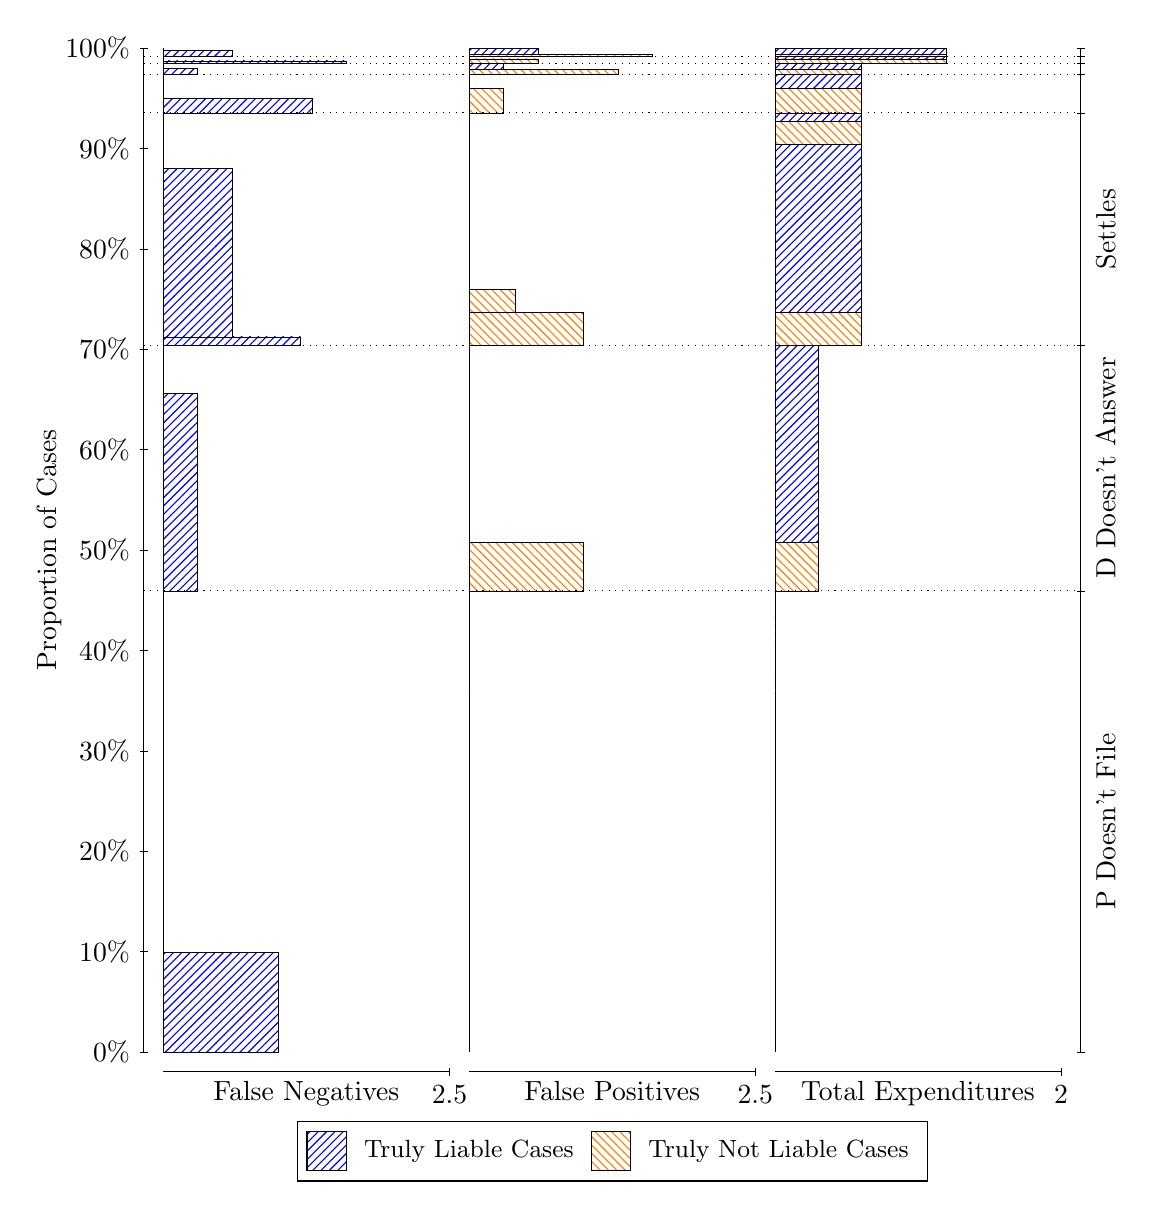
\begin{tikzpicture}
\draw[black, very thin] (1.5,1.75) -- (1.5,14.5);
\node[rotate=90, text=black, anchor=center] at (0.3, 8.125) {Proportion of Cases};
\draw[black, very thin] (1.45,1.75) -- (1.55,1.75);
\node[text=black, anchor=east] at (1.45, 1.75) {0\%};
\draw[black, very thin] (1.45,3.025) -- (1.55,3.025);
\node[text=black, anchor=east] at (1.45, 3.025) {10\%};
\draw[black, very thin] (1.45,4.3) -- (1.55,4.3);
\node[text=black, anchor=east] at (1.45, 4.3) {20\%};
\draw[black, very thin] (1.45,5.575) -- (1.55,5.575);
\node[text=black, anchor=east] at (1.45, 5.575) {30\%};
\draw[black, very thin] (1.45,6.85) -- (1.55,6.85);
\node[text=black, anchor=east] at (1.45, 6.85) {40\%};
\draw[black, very thin] (1.45,8.125) -- (1.55,8.125);
\node[text=black, anchor=east] at (1.45, 8.125) {50\%};
\draw[black, very thin] (1.45,9.4) -- (1.55,9.4);
\node[text=black, anchor=east] at (1.45, 9.4) {60\%};
\draw[black, very thin] (1.45,10.675) -- (1.55,10.675);
\node[text=black, anchor=east] at (1.45, 10.675) {70\%};
\draw[black, very thin] (1.45,11.95) -- (1.55,11.95);
\node[text=black, anchor=east] at (1.45, 11.95) {80\%};
\draw[black, very thin] (1.45,13.225) -- (1.55,13.225);
\node[text=black, anchor=east] at (1.45, 13.225) {90\%};
\draw[black, very thin] (1.45,14.5) -- (1.55,14.5);
\node[text=black, anchor=east] at (1.45, 14.5) {100\%};

\draw[black, very thin] (13.4,1.75) -- (13.4,14.5);
\draw[black, very thin] (13.35,1.75) -- (13.45,1.75);
\node[anchor=west] at (13.35, 1.75) {};
\draw[black, very thin] (13.35,7.6061) -- (13.45,7.6061);
\node[anchor=west] at (13.35, 7.6061) {};
\draw[black, very thin] (13.35,10.727) -- (13.45,10.727);
\node[anchor=west] at (13.35, 10.727) {};
\draw[black, very thin] (13.35,13.677) -- (13.45,13.677);
\node[anchor=west] at (13.35, 13.677) {};
\draw[black, very thin] (13.35,14.167) -- (13.45,14.167);
\node[anchor=west] at (13.35, 14.167) {};
\draw[black, very thin] (13.35,14.306) -- (13.45,14.306);
\node[anchor=west] at (13.35, 14.306) {};
\draw[black, very thin] (13.35,14.393) -- (13.45,14.393);
\node[anchor=west] at (13.35, 14.393) {};
\draw[black, very thin] (13.35,14.5) -- (13.45,14.5);
\node[anchor=west] at (13.35, 14.5) {};

\draw[black, very thin, pattern color=blue, pattern=north east lines] (1.75,1.75) rectangle (3.2033,3.0123);
\draw[black, very thin, pattern color=orange, pattern=north west lines] (1.75,3.0123) rectangle (1.75,7.6061);
\draw[black, very thin, pattern color=blue, pattern=north east lines] (1.75,7.6061) rectangle (2.186,10.113);
\draw[black, very thin, pattern color=orange, pattern=north west lines] (1.75,10.113) rectangle (1.75,10.727);
\draw[black, very thin, pattern color=blue, pattern=north east lines] (1.75,10.727) rectangle (3.494,10.831);
\draw[black, very thin, pattern color=blue, pattern=north east lines] (1.75,10.831) rectangle (2.622,12.97);
\draw[black, very thin, pattern color=orange, pattern=north west lines] (1.75,12.97) rectangle (1.75,13.677);
\draw[black, very thin, pattern color=blue, pattern=north east lines] (1.75,13.677) rectangle (3.6393,13.859);
\draw[black, very thin, pattern color=orange, pattern=north west lines] (1.75,13.859) rectangle (1.75,14.167);
\draw[black, very thin, pattern color=blue, pattern=north east lines] (1.75,14.167) rectangle (2.186,14.239);
\draw[black, very thin, pattern color=orange, pattern=north west lines] (1.75,14.239) rectangle (1.75,14.306);
\draw[black, very thin, pattern color=blue, pattern=north east lines] (1.75,14.306) rectangle (4.0753,14.338);
\draw[black, very thin, pattern color=orange, pattern=north west lines] (1.75,14.338) rectangle (1.75,14.393);
\draw[black, very thin, pattern color=blue, pattern=north east lines] (1.75,14.393) rectangle (2.622,14.468);
\draw[black, very thin, pattern color=orange, pattern=north west lines] (1.75,14.468) rectangle (1.75,14.5);
\draw[black, very thin, pattern color=orange, pattern=north west lines] (5.6333,1.75) rectangle (5.6333,6.3438);
\draw[black, very thin, pattern color=blue, pattern=north east lines] (5.6333,6.3438) rectangle (5.6333,7.6061);
\draw[black, very thin, pattern color=orange, pattern=north west lines] (5.6333,7.6061) rectangle (7.0867,8.2196);
\draw[black, very thin, pattern color=blue, pattern=north east lines] (5.6333,8.2196) rectangle (5.6333,10.727);
\draw[black, very thin, pattern color=orange, pattern=north west lines] (5.6333,10.727) rectangle (7.0867,11.138);
\draw[black, very thin, pattern color=orange, pattern=north west lines] (5.6333,11.138) rectangle (6.2147,11.434);
\draw[black, very thin, pattern color=blue, pattern=north east lines] (5.6333,11.434) rectangle (5.6333,13.677);
\draw[black, very thin, pattern color=orange, pattern=north west lines] (5.6333,13.677) rectangle (6.0693,13.984);
\draw[black, very thin, pattern color=blue, pattern=north east lines] (5.6333,13.984) rectangle (5.6333,14.167);
\draw[black, very thin, pattern color=orange, pattern=north west lines] (5.6333,14.167) rectangle (7.5227,14.233);
\draw[black, very thin, pattern color=blue, pattern=north east lines] (5.6333,14.233) rectangle (6.0693,14.306);
\draw[black, very thin, pattern color=orange, pattern=north west lines] (5.6333,14.306) rectangle (6.5053,14.361);
\draw[black, very thin, pattern color=blue, pattern=north east lines] (5.6333,14.361) rectangle (5.6333,14.393);
\draw[black, very thin, pattern color=orange, pattern=north west lines] (5.6333,14.393) rectangle (7.9587,14.424);
\draw[black, very thin, pattern color=blue, pattern=north east lines] (5.6333,14.424) rectangle (6.5053,14.5);
\draw[black, very thin, pattern color=orange, pattern=north west lines] (9.5167,1.75) rectangle (9.5167,6.3438);
\draw[black, very thin, pattern color=blue, pattern=north east lines] (9.5167,6.3438) rectangle (9.5167,7.6061);
\draw[black, very thin, pattern color=orange, pattern=north west lines] (9.5167,7.6061) rectangle (10.062,8.2196);
\draw[black, very thin, pattern color=blue, pattern=north east lines] (9.5167,8.2196) rectangle (10.062,10.727);
\draw[black, very thin, pattern color=orange, pattern=north west lines] (9.5167,10.727) rectangle (10.607,11.138);
\draw[black, very thin, pattern color=blue, pattern=north east lines] (9.5167,11.138) rectangle (10.607,13.277);
\draw[black, very thin, pattern color=orange, pattern=north west lines] (9.5167,13.277) rectangle (10.607,13.573);
\draw[black, very thin, pattern color=blue, pattern=north east lines] (9.5167,13.573) rectangle (10.607,13.677);
\draw[black, very thin, pattern color=orange, pattern=north west lines] (9.5167,13.677) rectangle (10.607,13.984);
\draw[black, very thin, pattern color=blue, pattern=north east lines] (9.5167,13.984) rectangle (10.607,14.167);
\draw[black, very thin, pattern color=orange, pattern=north west lines] (9.5167,14.167) rectangle (10.607,14.233);
\draw[black, very thin, pattern color=blue, pattern=north east lines] (9.5167,14.233) rectangle (10.607,14.306);
\draw[black, very thin, pattern color=orange, pattern=north west lines] (9.5167,14.306) rectangle (11.697,14.361);
\draw[black, very thin, pattern color=blue, pattern=north east lines] (9.5167,14.361) rectangle (11.697,14.393);
\draw[black, very thin, pattern color=orange, pattern=north west lines] (9.5167,14.393) rectangle (11.697,14.424);
\draw[black, very thin, pattern color=blue, pattern=north east lines] (9.5167,14.424) rectangle (11.697,14.5);
\draw[black, dotted] (1.5,7.6061) -- (13.4,7.6061);
\draw[black, dotted] (1.5,10.727) -- (13.4,10.727);
\draw[black, dotted] (1.5,13.677) -- (13.4,13.677);
\draw[black, dotted] (1.5,14.167) -- (13.4,14.167);
\draw[black, dotted] (1.5,14.306) -- (13.4,14.306);
\draw[black, dotted] (1.5,14.393) -- (13.4,14.393);
\draw[black, very thin] (1.75,1.5) -- (5.3833,1.5);
\node[text=black, anchor=north] at (3.5667, 1.5) {False Negatives};
\draw[black, very thin] (5.3833,1.45) -- (5.3833,1.55);
\node[text=black, anchor=north] at (5.3833, 1.45) {2.5};

\draw[black, very thin] (5.6333,1.5) -- (9.2667,1.5);
\node[text=black, anchor=north] at (7.45, 1.5) {False Positives};
\draw[black, very thin] (9.2667,1.45) -- (9.2667,1.55);
\node[text=black, anchor=north] at (9.2667, 1.45) {2.5};

\draw[black, very thin] (9.5167,1.5) -- (13.15,1.5);
\node[text=black, anchor=north] at (11.333, 1.5) {Total Expenditures};
\draw[black, very thin] (13.15,1.45) -- (13.15,1.55);
\node[text=black, anchor=north] at (13.15, 1.45) {2};

\node[text=black, centered, rotate=90] at (13.72, 4.6781) {P Doesn't File};
\node[text=black, centered, rotate=90] at (13.72, 9.1666) {D Doesn't Answer};
\node[text=black, centered, rotate=90] at (13.72, 12.202) {Settles};





\draw (7.449999999999999,1.5) node[draw=none] (baseCoordinate) {};
\begin{scope}[align=center]
        \matrix[scale=0.5, draw=black, below=0.5cm of baseCoordinate, nodes={draw}, column sep=0.1cm]{
            \node[rectangle, draw, minimum width=0.5cm, minimum height=0.5cm, pattern color=blue, pattern=north east lines] {}; &
            \node[draw=none, font=\small, text=black] (B) {Truly Liable Cases}; &
            \node[rectangle, draw, minimum width=0.5cm, minimum height=0.5cm, pattern color=orange, pattern=north west lines] {}; &
            \node[draw=none, font=\small, text=black] (B) {Truly Not Liable Cases}; \\
            };
\end{scope}

\end{tikzpicture}
\end{document}